\documentclass{beamer}
\usepackage[utf8]{inputenc}

\usetheme{Madrid}
\usecolortheme{default}
\usepackage{amsmath,amssymb,amsfonts,amsthm}
\usepackage{txfonts}
\usepackage{tkz-euclide}
\usepackage{listings}
\usepackage{adjustbox}
\usepackage{array}
\usepackage{tabularx}
\usepackage{gvv}
\usepackage{lmodern}
\usepackage{circuitikz}
\usepackage{tikz}
\usepackage{graphicx}
\usepackage{multicol}
\usepackage{enumitem}

\setbeamertemplate{page number in head/foot}[totalframenumber]

\usepackage{tcolorbox}
\tcbuselibrary{minted,breakable,xparse,skins}

\definecolor{bg}{gray}{0.95}
\DeclareTCBListing{mintedbox}{O{}m!O{}}{%
  breakable=true,
  listing engine=minted,
  listing only,
  minted language=#2,
  minted style=default,
  minted options={%
    linenos,
    gobble=0,
    breaklines=true,
    breakafter=,,
    fontsize=\small,
    numbersep=8pt,
    #1},
  boxsep=0pt,
  left skip=0pt,
  right skip=0pt,
  left=25pt,
  right=0pt,
  top=3pt,
  bottom=3pt,
  arc=5pt,
  leftrule=0pt,
  rightrule=0pt,
  bottomrule=2pt,
  toprule=2pt,
  colback=bg,
  colframe=orange!70,
  enhanced,
  overlay={%
    \begin{tcbclipinterior}
    \fill[orange!20!white] (frame.south west) rectangle ([xshift=20pt]frame.north west);
    \end{tcbclipinterior}},
  #3,
}
\lstset{
    language=C,
    basicstyle=\ttfamily\small,
    keywordstyle=\color{blue},
    stringstyle=\color{orange},
    commentstyle=\color{green!60!black},
    numbers=left,
    numberstyle=\tiny\color{gray},
    breaklines=true,
    showstringspaces=false,
}

\numberwithin{equation}{section}
\lstset{
  language=Python,
  basicstyle=\ttfamily\small,
  keywordstyle=\color{blue},
  stringstyle=\color{orange},
  numbers=left,
  numberstyle=\tiny\color{gray},
  breaklines=true,
  showstringspaces=false
}


\title{Problem 2.10.20.}
\author{Sarvesh Tamgade}

\date{\today} 
\begin{document}

\begin{frame}
\titlepage
\end{frame}
\section{Question}
\begin{frame}{Question}
\textbf{Question}:
 Which of the following expressions are meaningful?
\begin{multicols}{2}
\begin{enumerate}[label=(\alph*)]
     
\item $\vec{u} \cdot (\vec{v} \times \vec{w})$
\item $(\vec{u} \cdot \vec{v}) \cdot \vec{w}$
\item $(\vec{u} \cdot \vec{v})\ \vec{w}$
\item $\vec{u} \times (\vec{v} \cdot \vec{w})$

\end{enumerate}
\end{multicols}
\end{frame}

\section{Solution}
\begin{frame}[fragile]
    \frametitle{Solution}
Let
\begin{align}
    \vec{u} &= \myvec{2 \\ 3}, \quad
    \vec{v} = \myvec{4 \\ 1}, \quad
    \vec{w} = \myvec{0 \\ 5}.
\end{align}

\begin{enumerate}[label=\alph*)]
  \item \( \vec{u}^\top (\vec{v} \times \vec{w}) \)
  
\[
\vec{v} \times \vec{w} =
\myvec{
v_{23} & w_{23} \\
v_{31} & w_{31} \\
v_{12} & w_{12}
}
=
\myvec{
v_2 w_3 - v_3 w_2 \\
v_3 w_1 - v_1 w_3 \\
v_1 w_2 - v_2 w_1
}
=
\myvec{
1 \times 0 - 0 \times 5 \\
0 \times 0 - 4 \times 0 \\
4 \times 5 - 1 \times 0
}
=
\myvec{
0 \\
0 \\
20
}
\]

\end{enumerate}
\end{frame}
\begin{frame}[fragile]
    \frametitle{Solution}
\begin{enumerate}[label=\alph*) ]
\setcounter{enumi}{1} 
 
\[
\vec{u}^\top (\vec{v} \times \vec{w}) =
\myvec{2 & 3 & 0}  % row vector (transpose of u)
\myvec{
0 \\
0 \\
20
}
= 0
\]

Since the scalar (dot) product of two vectors is defined, the expression  \(\vec{u}^\top(\vec{v} \times \vec{w})\) is meaningful.

  \item \( (\vec{u}^\top \vec{v})^\top \vec{w} \)

  \begin{align*}
  \vec{u}^\top \vec{v} &= \myvec{2 & 3} \myvec{4 \\ 1} = 2 \times 4 + 3 \times 1 = 11,
  \\
  (\vec{u}^\top \vec{v})^\top \vec{w} &= 11^\top \myvec{0 \\ 5} \quad \text{(scalar dot vector -- undefined)}.
  \end{align*}

  \item \( (\vec{u}^\top \vec{v}) \vec{w} \)
  
\end{enumerate}

\end{frame}
\begin{frame}[fragile]
    \frametitle{Solution}
\begin{enumerate}[label=\alph*) ]
\setcounter{enumi}{3} 
 

  \begin{align*}
  (\vec{u}^\top \vec{v}) \vec{w} &= 11 \times \myvec{0 \\ 5} = \myvec{0 \\ 55}.
  \end{align*}
  
  This is meaningful scalar multiplication.

  \item \( \vec{u} \times (\vec{v}^\top \vec{w}) \)
  
  \begin{align*}
  \vec{v}^\top \vec{w} &= \myvec{4 & 1} \myvec{0 \\ 5} = 0 + 5 = 5,
  \\
  \vec{u} \times 5 &= \text{cross product of vector and scalar -- undefined}.
  \end{align*}

\end{enumerate}

\textbf{Answer:}
\boxed{\text{Only (a) and (c) are meaningful }}

\end{frame}
\section{Graph}
\begin{frame}
    \frametitle{Graph}
    \begin{figure}[htbp]
    \centering
    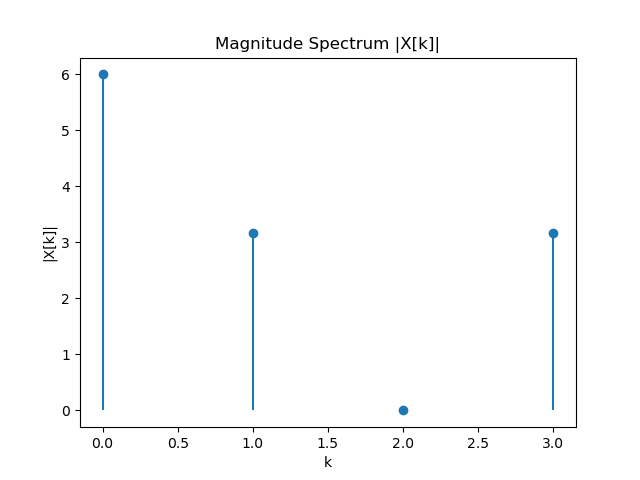
\includegraphics[width=0.65\linewidth]{FIG/fig1.png}
    \caption{Vector Representation}
    \label{fig:FIG/fig1.png}
\end{figure}
\end{frame}
\section{ C Code}
\begin{frame}[fragile]
\frametitle{C Code }
\begin{lstlisting}[language=C]
#include <stdio.h>
#include "matfun.h"

void print_vector(const char* name, const double v[3]) {
    printf("%s = (%.2f, %.2f, %.2f)\n", name, v[0], v[1], v[2]);
}

int main() {
    double u[3] = {1, 2, 3};
    double v[3] = {4, 5, 6};
    double w[3] = {7, 8, 9};

    double cross_vw[3];
    cross_product(v, w, cross_vw);

    double dot_u_crossvw = dot_product(u, cross_vw);
    printf("u · (v × w) = %.2f\n", dot_u_crossvw);


   
    
\end{lstlisting}
\end{frame}
\begin{frame}[fragile]
\frametitle{C Code }
\begin{lstlisting}[language=C]
 double dot_uv = dot_product(u, v);
    printf("(u · v) = %.2f\n", dot_uv);

    printf("(u · v) · w is NOT meaningful as dot product of scalar and vector.\n");

    printf("(u · v) * w (scalar multiplication) = (%.2f, %.2f, %.2f)\n",
           dot_uv * w[0], dot_uv * w[1], dot_uv * w[2]);

    printf("v · w = %.2f\n", dot_product(v, w));
    printf("u × (v · w) is NOT meaningful as cross product of vector and scalar.\n");

    return 0;
}


\end{lstlisting}
\end{frame}

\begin{frame}[fragile]
\frametitle{Python Code for Plotting}
\begin{lstlisting}[language=Python]
import matplotlib.pyplot as plt
import numpy as np

# Vectors u, v, w in 2D (using first two components)
u = np.array([2, 3])
v = np.array([4, 1])
w = np.array([0, 5])

# Origin point
origin = np.array([0, 0])

# Plotting the vectors
plt.figure(figsize=(7, 7))
plt.quiver(*origin, *u, angles='xy', scale_units='xy', scale=1, color='red', label='u = [2, 3]')
plt.quiver(*origin, *v, angles='xy', scale_units='xy', scale=1, color='green', label='v = [4, 1]')
plt.quiver(*origin, *w, angles='xy', scale_units='xy', scale=1, color='blue', label='w = [0, 5]')

\end{lstlisting}

\end{frame}
\begin{frame}[fragile]
\frametitle{Python Code for Plotting}
\begin{lstlisting}[language=Python]
# Setting the limits
plt.xlim(-1, 5)
plt.ylim(-1, 6)

# Adding labels and title
plt.xlabel('X')
plt.ylabel('Y')
plt.title('2D vectors: u, v, w')
plt.grid()
plt.legend()
plt.gca().set_aspect('equal')

# Save the figure as a PNG file
plt.savefig('2D_vectors.png')
plt.close()end{lstlisting}

\end{lstlisting}

\end{frame}

\end{document}
